% Slides — Capítulo 11: Circulação Geral
\documentclass[aspectratio=169,11pt]{beamer}
\usepackage{../comum/temameteo}
\graphicspath{{../figuras/cap11/}}

\title[Cap. 11 --- Circulação Geral]{Capítulo 11 --- Circulação Geral}
\subtitle{Meteorologia Prática}
\author{}
\date{}

\begin{document}

\begin{frame}
  \titlepage
  \vfill
  \atribuicao
\end{frame}

\begin{frame}{Roteiro}
  \tableofcontents
\end{frame}

% ---------------------------------------------------------------
\section{O motor: aquecimento diferencial}

\begin{frame}{Trópicos lucram, polos pagam}
  \begin{columns}
    \column{0.4\textwidth}
    \begin{itemize}
      \item Absorvida: pico no equador (Cap.~2). OLR: quase plana.
      \item A OLR é plana \alert{porque} a circulação já espalhou a
            energia.
      \item Superávit tropical $+$ déficit polar $\Rightarrow$
            transporte obrigatório.
    \end{itemize}
    \column{0.6\textwidth}
    \figlivroslide{fig_11_12.jpg}{0.52\textheight}{Fig.~11.12 ---
      superávit e déficit radiativo por latitude}
  \end{columns}
\end{frame}

\begin{frame}{O transporte exigido: 5 PW}
  \begin{columns}
    \column{0.4\textwidth}
    \eqdestaque{$T(\phi) = \displaystyle\int_{-90°}^{\phi}
      (Q_{abs}-OLR)\,2\pi R^2\cos\phi'\,d\phi'$}
    \vspace{0.4em}
    \begin{itemize}
      \item Pico $\sim$5--6\,PW perto de $35°$ ($\sim$70$\times$ o
            consumo elétrico mundial).
      \item Teste: $T(90°) = 0$ (T1). Cálculo no Caso~1.
      \item Atmosfera $\sim$4\,PW $+$ oceano $\sim$1--2\,PW.
    \end{itemize}
    \column{0.6\textwidth}
    \figlivroslide{fig_11_14.jpg}{0.5\textheight}{Fig.~11.14 ---
      transporte total e as parcelas atmosfera/oceano}
  \end{columns}
\end{frame}

\begin{frame}{O transporte no notebook}
  \begin{columns}
    \column{0.4\textwidth}
    \begin{itemize}
      \item Insolação do Cap.~2 $+$ albedo $\phi$-dependente $+$ OLR
            quase plana.
      \item Pico: 22\,PW? Não — 22\,PW é o que \emph{daria} sem
            oceano/ajustes; a curva certa fecha em $\pm$5--6\,PW por
            hemisfério.
      \item N1: gelo polar ($A=0{,}6$) aumenta o transporte exigido —
            gostinho de feedback (Cap.~21).
    \end{itemize}
    \column{0.6\textwidth}
    \begin{center}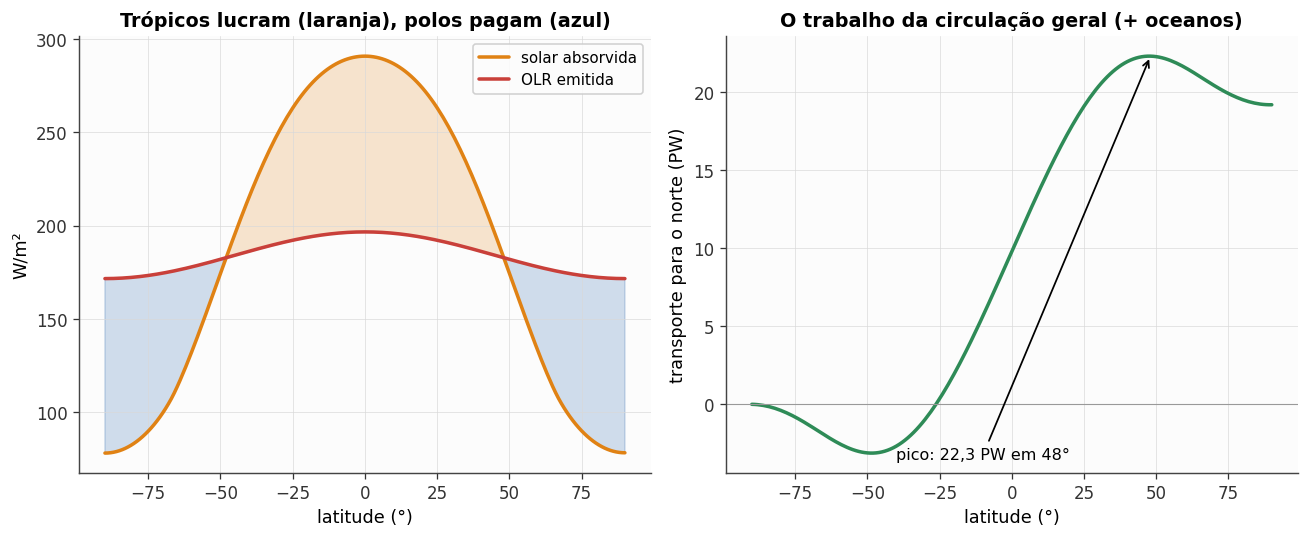
\includegraphics[width=0.95\linewidth]{notebook_transporte.png}\\[-2pt]
    {\tiny desequilíbrio radiativo e transporte exigido — Caso~1 do notebook do curso}\end{center}
  \end{columns}
\end{frame}

% ---------------------------------------------------------------
\section{As três células}

\begin{frame}{As três células e os cinturões}
  \begin{columns}
    \column{0.4\textwidth}
    \begin{itemize}
      \item \alert{Hadley} (0--30°): a célula térmica direta.
      \item Ferrel (30--60°): indireta, movida pelos turbilhões.
      \item Polar: rasa e fria.
      \item Entre elas: os jatos — e as ondas de Rossby.
    \end{itemize}
    \column{0.6\textwidth}
    \figlivroslide{fig_11_1c.jpg}{0.56\textheight}{Fig.~11.1 --- células
      de Hadley, ondas de Rossby e células polares}
  \end{columns}
\end{frame}

\begin{frame}{Hadley em corte: ZCIT, alísios, desertos}
  \begin{columns}
    \column{0.4\textwidth}
    \begin{itemize}
      \item Sobe na ZCIT (chuva diária — o cinturão do mapa do
            Cap.~7).
      \item Desce em $\sim$30°: Saara, Atacama, altas semifixas.
      \item Retorno $+$ Coriolis $=$ alísios de SE (HS).
      \item Acima dos alísios: a inversão que limita a convecção.
    \end{itemize}
    \column{0.6\textwidth}
    \figlivroslide{fig_11_27a.jpg}{0.52\textheight}{Fig.~11.27 --- a
      célula de Hadley em corte meridional}
  \end{columns}
\end{frame}

\begin{frame}{Momento angular fabrica o jato subtropical}
  \begin{columns}
    \column{0.44\textwidth}
    \eqdestaque{$u(\phi) = \Omega R\,\dfrac{\sin^2\phi}{\cos\phi}
      \;\Rightarrow\; u(30°) = 134$\,m/s}
    \vspace{0.4em}
    \begin{itemize}
      \item Anel que sai do equador conservando $M$ acelera para
            leste.
      \item Observado: $\sim$40\,m/s — turbilhões roubam o excesso
            (T2).
      \item A célula \alert{tem} que acabar em $\sim$30°: o jato que
            ela cria fica instável.
    \end{itemize}
    \column{0.56\textwidth}
    \figlivroslide{fig_11_43c.jpg}{0.48\textheight}{Fig.~11.43 ---
      conservação de momento angular no anel que migra}
  \end{columns}
\end{frame}

% ---------------------------------------------------------------
\section{Vento térmico e jatos}

\begin{frame}{A dedução mais elegante do curso}
  \begin{columns}
    \column{0.5\textwidth}
    \eqdestaque{$\dfrac{\partial u_g}{\partial z} =
      -\dfrac{g}{f\,T}\,\dfrac{\partial T}{\partial y}$}
    \vspace{0.4em}
    \begin{itemize}
      \item Geostrofia (Cap.~10) $+$ hidrostática (Cap.~1), uma
            derivada.
      \item Leitura: camada quente $=$ espessa (hipsométrica)
            $\Rightarrow$ superfícies de pressão inclinam mais com a
            altura $\Rightarrow$ vento cresce.
      \item Contraste de 5\,K/1000\,km em 10\,km: $+19$\,m/s.
    \end{itemize}
    \column{0.5\textwidth}
    \figlivroslide{fig_11_20.jpg}{0.5\textheight}{Fig.~11.20 ---
      espessura inclinando as superfícies de pressão: nasce o vento
      térmico}
  \end{columns}
\end{frame}

\begin{frame}{Espessura na carta $=$ vento térmico}
  \begin{columns}
    \column{0.4\textwidth}
    \begin{itemize}
      \item Carta de espessura 100--50\,kPa: o ``termômetro'' do
            Cap.~1 em campo.
      \item O vento térmico sopra \alert{paralelo às linhas de
            espessura}, ar frio à esquerda (HS: à direita).
      \item Advecções quente/fria lidas num relance (Cap.~12).
    \end{itemize}
    \column{0.6\textwidth}
    \figlivroslide{fig_11_21.jpg}{0.54\textheight}{Fig.~11.21 ---
      espessura 100--50\,kPa e vetores de vento térmico}
  \end{columns}
\end{frame}

\begin{frame}{Os dois jatos}
  \begin{columns}
    \column{0.4\textwidth}
    \begin{itemize}
      \item \alert{Subtropical} ($\sim$30°, 12\,km): borda da Hadley,
            momento angular.
      \item \alert{Polar} (40--60°, 10\,km): vento térmico sobre a
            frente polar.
      \item Inverno: contraste maior $\Rightarrow$ jato mais forte e
            mais equatorial — a temporada de tempestades (Cap.~13).
    \end{itemize}
    \column{0.6\textwidth}
    \figlivroslide{fig_11_35b.jpg}{0.52\textheight}{Fig.~11.35 ---
      posição dos jatos e células no inverno}
  \end{columns}
\end{frame}

\begin{frame}{O jato em números}
  \begin{columns}
    \column{0.4\textwidth}
    \begin{itemize}
      \item Núcleo de 30--50\,m/s (inverno), $\sim$10--12\,km.
      \item Turbulência de céu claro nas bordas: cisalhamento $+$
            $Ri < 0{,}25$ (Cap.~5).
      \item Caso~4 do notebook: vento térmico integrado num perfil
            realista — o jato aparece sozinho.
    \end{itemize}
    \column{0.6\textwidth}
    \figlivroslide{fig_11_37a.jpg}{0.52\textheight}{Fig.~11.37 --- vento
      zonal médio em corte meridional: os jatos}
  \end{columns}
\end{frame}

% ---------------------------------------------------------------
\section{Ondas de Rossby}

\begin{frame}{A mola $\beta$: o planeta redondo é o meio elástico}
  \begin{columns}
    \column{0.44\textwidth}
    \eqdestaque{$c = U - \dfrac{\beta}{k^2}$,\qquad
      $\beta = \dfrac{2\Omega\cos\phi}{R}$}
    \vspace{0.4em}
    \begin{itemize}
      \item Parcela deslocada muda $f$, gira, volta: conservação de
            $\zeta + f$.
      \item Ondas longas andam para \alert{oeste} contra o jato.
      \item Estacionária: $\lambda_s = 2\pi\sqrt{U/\beta} \sim
            6000$\,km $\Rightarrow$ 4--5 meandros no HS.
    \end{itemize}
    \column{0.56\textwidth}
    \figlivroslide{fig_11_51a.jpg}{0.5\textheight}{Fig.~11.51 --- o
      mecanismo de restauração no plano $\beta$}
  \end{columns}
\end{frame}

\begin{frame}{Meandros que fazem o tempo}
  \begin{columns}
    \column{0.4\textwidth}
    \begin{itemize}
      \item Cristas e cavados das ondas $=$ altas e baixas móveis
            (Cap.~13).
      \item Onda amplificada que ``quebra'': bloqueios, ondas de
            calor/frio persistentes (Cap.~21).
      \item Dispersão e onda estacionária: Caso~3 do notebook.
    \end{itemize}
    \column{0.6\textwidth}
    \figlivroslide{fig_11_49b.jpg}{0.52\textheight}{Fig.~11.49 --- o
      vórtice polar ondulado pelas ondas planetárias}
  \end{columns}
\end{frame}

% ---------------------------------------------------------------
\section{O retrato completo}

\begin{frame}{Cinturões de pressão e ventos à superfície}
  \begin{columns}
    \column{0.4\textwidth}
    \begin{itemize}
      \item ZCIT $\cdot$ altas subtropicais $\cdot$ oestes das
            latitudes médias $\cdot$ altas polares.
      \item Alísios convergindo na ZCIT; oestes carregando os
            ciclones em fila.
      \item Compare com o mapa real de janeiro/julho (monções:
            Cap.~11 do livro).
    \end{itemize}
    \column{0.6\textwidth}
    \figlivroslide{fig_11_3a.jpg}{0.54\textheight}{Fig.~11.3 --- o
      planeta idealizado: células, cinturões e ventos}
  \end{columns}
\end{frame}

\begin{frame}{O mapa do capítulo}
  \eqdestaque{$Q_{abs}-OLR \to T(\phi)\ (5\,\mathrm{PW}) \to
    \text{Hadley} + \text{jato subtropical} \to
    \partial_z u_g = -\tfrac{g}{fT}\partial_y T \to
    c = U - \beta/k^2$}
  \vspace{0.6em}
  Um desequilíbrio radiativo, três células, dois jatos e uma família de
  ondas: o esqueleto de todo o tempo do planeta. Daqui o curso desce de
  escala: massas de ar e frentes (Cap.~12), ciclones (Cap.~13).
\end{frame}

\begin{frame}{Laboratório numérico --- notebook do Cap.~11}
  \texttt{notebooks/cap11\_circulacao.ipynb}
  \begin{enumerate}
    \item Desequilíbrio radiativo $\to$ transporte exigido (os 5\,PW).
    \item EBM meridional com \texttt{climlab}: $T(\phi)$ e a linha do
          gelo.
    \item Dispersão de Rossby e a onda estacionária.
    \item Vento térmico $\to$ o jato numa seção meridional.
  \end{enumerate}
  \vspace{0.4em}
  \textbf{Exercícios}: T1--T5 e N1--N4 nas notas; células reservadas no
  notebook.
  \vfill
  \atribuicao
\end{frame}

\end{document}
